\chapter{Behandelte Algorithmen und ihre theoretische Effizienz}
\label{cha:algorithmen}

In diesem Kapitel werden die in der folgenden Arbeit behandelten Sortieralgorithmen mit ihrer theoretischen Effizienz dargelegt.

Konkrete Implementation der folgenden Algorithmen sind \prettyref{app:implementations} zu entnehmen.

\section{Insertionsort}
\label{sec:alg-insertion}

Wie schon in \prettyref{sec:sorting-algorithms-definition} ausgeführt, baut der Insertionsort auf der Annahme auf, dass vor der Begutachtung eines Elements $A[j]$ die Elemente $A[1 \twodots j - 1]$ bereits sortiert wurden. $A[j]$ wird anschließend in das bereits sortierte \enquote{Subarray} einsortiert (vgl. \cite[80]{taocp3}). Siehe \prettyref{fig:insertions-example} für eine Illustration der Vorgehensweise anhand eines Beispielarrays.

\begin{codebox}
    \Procname{$\text{Insertionsort}(A)$}
    \li \For $j \gets 2$ \To $\attrib{A}{length}$\label{ln:insertions-for-begin}
    \li     \Do\label{ln:ins-for-body-begin}
                $\id{key} \gets A[j]$\label{ln:ins-intermediary}
    \li         \Comment Insert $A[j]$ into the sorted sequence $A[1 \twodots j-1]$.
    \li         $i \gets j-1$\label{ln:ins-initial-i}
    \li         \While $i > 0$ and $A[i] > \id{key}$ \label{ln:ins-inner-while}
    \li             \Do
                        $A[i+1] \gets A[i]$\label{ln:ins-value-move}
    \li                 $i \gets i-1$
                    \End
    \li         $A[i+1] \gets \id{key}$\label{ln:ins-insertion}
            \End\label{ln:insertions-for-end}
\end{codebox}

\begin{figure}[hbt]
    \centering
    \begin{subfigure}{.3\linewidth}
        \centering

        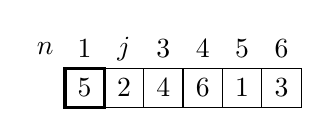
\begin{tikzpicture}
            \draw [very thick] (0.0, 0.0) rectangle (0.5, 0.5) node[midway]{5};
            \draw [] (0.5, 0.0) rectangle (1.0, 0.5) node[midway]{2};
            \draw [] (1.0, 0.0) rectangle (1.5, 0.5) node[midway]{4};
            \draw [] (1.5, 0.0) rectangle (2.0, 0.5) node[midway]{6};
            \draw [] (2.0, 0.0) rectangle (2.5, 0.5) node[midway]{1};
            \draw [] (2.5, 0.0) rectangle (3.0, 0.5) node[midway]{3};
            
            \path   node at (-0.25, 0.75) [] {$n$}
                    node at (0.25, 0.75) [] {1}
                    node at (0.75, 0.75) [] {$j$}
                    node at (1.25, 0.75) [] {3}
                    node at (1.75, 0.75) [] {4}
                    node at (2.25, 0.75) [] {5}
                    node at (2.75, 0.75) [] {6};
        \end{tikzpicture}

        \caption{\label{fig:insertions-example-begin}}
    \end{subfigure}
    \hfill
    \begin{subfigure}{.3\linewidth}
        \centering
        
        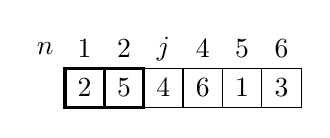
\begin{tikzpicture}
            \draw [very thick] (0.0, 0.0) rectangle (0.5, 0.5) node[midway]{2};
            \draw [very thick] (0.5, 0.0) rectangle (1.0, 0.5) node[midway]{5};
            \draw [] (1.0, 0.0) rectangle (1.5, 0.5) node[midway]{4};
            \draw [] (1.5, 0.0) rectangle (2.0, 0.5) node[midway]{6};
            \draw [] (2.0, 0.0) rectangle (2.5, 0.5) node[midway]{1};
            \draw [] (2.5, 0.0) rectangle (3.0, 0.5) node[midway]{3};
            
            \path   node at (-0.25, 0.75) [] {$n$}
                    node at (0.25, 0.75) [] {1}
                    node at (0.75, 0.75) [] {2}
                    node at (1.25, 0.75) [] {$j$}
                    node at (1.75, 0.75) [] {4}
                    node at (2.25, 0.75) [] {5}
                    node at (2.75, 0.75) [] {6};
        \end{tikzpicture}
        
        \caption{}
    \end{subfigure}
    \hfill
    \begin{subfigure}{.3\linewidth}
        \centering
        
        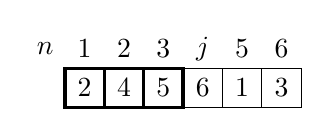
\begin{tikzpicture}
            \draw [very thick] (0.0, 0.0) rectangle (0.5, 0.5) node[midway]{2};
            \draw [very thick] (0.5, 0.0) rectangle (1.0, 0.5) node[midway]{4};
            \draw [very thick] (1.0, 0.0) rectangle (1.5, 0.5) node[midway]{5};
            \draw [] (1.5, 0.0) rectangle (2.0, 0.5) node[midway]{6};
            \draw [] (2.0, 0.0) rectangle (2.5, 0.5) node[midway]{1};
            \draw [] (2.5, 0.0) rectangle (3.0, 0.5) node[midway]{3};
            
            \path   node at (-0.25, 0.75) [] {$n$}
                    node at (0.25, 0.75) [] {1}
                    node at (0.75, 0.75) [] {2}
                    node at (1.25, 0.75) [] {3}
                    node at (1.75, 0.75) [] {$j$}
                    node at (2.25, 0.75) [] {5}
                    node at (2.75, 0.75) [] {6};
        \end{tikzpicture}

        \caption{}
    \end{subfigure}

    \bigskip
    \begin{subfigure}{.3\linewidth}
        \centering
        
        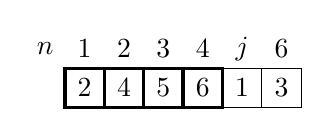
\begin{tikzpicture}
            \draw [very thick] (0.0, 0.0) rectangle (0.5, 0.5) node[midway]{2};
            \draw [very thick] (0.5, 0.0) rectangle (1.0, 0.5) node[midway]{4};
            \draw [very thick] (1.0, 0.0) rectangle (1.5, 0.5) node[midway]{5};
            \draw [very thick] (1.5, 0.0) rectangle (2.0, 0.5) node[midway]{6};
            \draw [] (2.0, 0.0) rectangle (2.5, 0.5) node[midway]{1};
            \draw [] (2.5, 0.0) rectangle (3.0, 0.5) node[midway]{3};
            
            \path   node at (-0.25, 0.75) [] {$n$}
                    node at (0.25, 0.75) [] {1}
                    node at (0.75, 0.75) [] {2}
                    node at (1.25, 0.75) [] {3}
                    node at (1.75, 0.75) [] {4}
                    node at (2.25, 0.75) [] {$j$}
                    node at (2.75, 0.75) [] {6};
        \end{tikzpicture}
        
        \caption{}
    \end{subfigure}
    \hfill
    \begin{subfigure}{.3\linewidth}
        \centering
        
        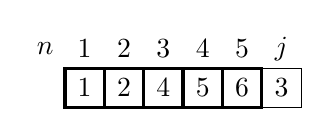
\begin{tikzpicture}
            \draw [very thick] (0.0, 0.0) rectangle (0.5, 0.5) node[midway]{1};
            \draw [very thick] (0.5, 0.0) rectangle (1.0, 0.5) node[midway]{2};
            \draw [very thick] (1.0, 0.0) rectangle (1.5, 0.5) node[midway]{4};
            \draw [very thick] (1.5, 0.0) rectangle (2.0, 0.5) node[midway]{5};
            \draw [very thick] (2.0, 0.0) rectangle (2.5, 0.5) node[midway]{6};
            \draw [] (2.5, 0.0) rectangle (3.0, 0.5) node[midway]{3};

            \path   node at (-0.25, 0.75) [] {$n$}
                    node at (0.25, 0.75) [] {1}
                    node at (0.75, 0.75) [] {2}
                    node at (1.25, 0.75) [] {3}
                    node at (1.75, 0.75) [] {4}
                    node at (2.25, 0.75) [] {5}
                    node at (2.75, 0.75) [] {$j$};
        \end{tikzpicture}

        \caption{\label{fig:insertions-example-end}}
    \end{subfigure}
    \hfill
    \begin{subfigure}{.3\linewidth}
        \centering
        
        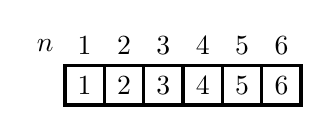
\begin{tikzpicture}
            \draw [very thick] (0.0, 0.0) rectangle (0.5, 0.5) node[midway]{1};
            \draw [very thick] (0.5, 0.0) rectangle (1.0, 0.5) node[midway]{2};
            \draw [very thick] (1.0, 0.0) rectangle (1.5, 0.5) node[midway]{3};
            \draw [very thick] (1.5, 0.0) rectangle (2.0, 0.5) node[midway]{4};
            \draw [very thick] (2.0, 0.0) rectangle (2.5, 0.5) node[midway]{5};
            \draw [very thick] (2.5, 0.0) rectangle (3.0, 0.5) node[midway]{6};
            
            \path   node at (-0.25, 0.75) [] {$n$}
                    node at (0.25, 0.75) [] {1}
                    node at (0.75, 0.75) [] {2}
                    node at (1.25, 0.75) [] {3}
                    node at (1.75, 0.75) [] {4}
                    node at (2.25, 0.75) [] {5}
                    node at (2.75, 0.75) [] {6};
        \end{tikzpicture}
        \caption{\label{fig:insertions-example-final}}
    \end{subfigure}
    % Underfull hbox because of the first line
    \caption{Illustration des Arrays $A = \{5, 2, 4, 6, 1, 3\}$ während es von $\proc{Insertion-Sort}(A)$ bearbeitet wird. Über einem Rechteck steht sein Index in $A$, in den Rechtecken steht der jeweilige Wert von $A$ an diesem Index. Fett gedruckte Rechtecke sind Teil des bereits sortierten Subarrays $A[1 \twodots j - 1]$. \subref{fig:insertions-example-begin} bis \subref{fig:insertions-example-end} zeigen die fünf Iterationen der $\For$-Schleife auf Zeilen \ref{ln:insertions-for-begin}--\ref{ln:insertions-for-end} beginnend mit $j = 2$ bis $j = \attrib{A}{length}$ beziehungsweise $j = 6$. Das Element $A[j]$ ist mit einem Obenstehendem $j$ gekennzeichnet, in der jeweils nächsten Iteration wurde es dann bereits an seine korrekte Position im sortierten Subarray $A[1 \twodots j - 1]$ bewegt. \subref{fig:insertions-example-final} zeigt das sortierte Array. Abbildungen \subref{fig:insertions-example-begin} -- \subref{fig:insertions-example-end} sind maßgeblich inspiriert von \cite[18]{clrs2001}, Figure 2.2.}
    \label{fig:insertions-example}
\end{figure}


\text{Insertionsort} ist aus \cite[18]{clrs2001} entnommen, eine Implementation ist in \prettyref{lst:insertion} zu finden.

Im günstigsten Fall ist $A$ bereits sortiert, für alle $j = 2, 3, \twodots \attrib{A}{length}$ gilt nun $A[j - 1] \leq \id{key}$: der Körper der $\While$-Schleife auf \prettyref{ln:ins-inner-while} wird also nie ausgeführt. Der Algorithmus ist in diesem Fall in $O(n)$ (vgl. \cite[28]{clrs2001}).

Der ungünstigste Fall ist eine umgekehrt sortierte Liste. Jedes Element $A[j]$ muss mit jedem Element des sortierten Subarrays $A[1 \ldots i]$ verglichen werden, der Algorithmus ist in diesem Fall also in $O(n^2)$ (vgl. \cite[28f]{clrs2001}).

\section{Quicksort}
\label{sec:alg-exchanging}

Quicksort ist ein \emph{divide-and-conquer} Algorithmus, der rekursiv ein Array in zwei Subarrays teilt und diese sortiert (vgl. \cite[113f]{taocp3}). Ein Aufteilungs- bzw. Partitionsalgorithmus teilt ein Array $A[p \twodots r]$ in zwei Subarrays $A[p \twodots q-1]$ und $A[q + 1 \twodots r]$. Diese Teilung erfolgt derart, dass alle Elemente $A[p \twodots q-1]$ kleiner oder gleich $A[q]$ sind und alle Elemente $A[q+1 \twodots r]$ größer oder gleich $A[q]$ sind. Der Index $q$ wird als Teil der Prozedur ermittelt.

\begin{codebox}
    \Procname{$\text{Partition}(A, p, r)$}
    \li $x \gets A[r]$
    \li $i \gets p - 1$
    \li \For $j = p$ \To $r - 1$
    \li     \Do
                \If $A[j] \leq x$
    \li             \Then
                        $i \gets i + 1$
    \li                 exchange $A[i]$ with $A[j]$
                    \End
            \End
    \li exchange $A[i + 1]$ with $A[r]$
    \li \Return i + 1
\end{codebox}

$\text{Partition}$ wählt immer ein Element $x = A[r]$ als \enquote{Drehpunkt}, um den das Subarray $A[p \twodots r]$ geteilt wird. Im Laufe der Prozedur wird das Subarray in vier Regionen geteilt, die gewisse Eigenschaften erfüllten, zu sehen in \prettyref{fig:quicks-partitioning}.

\begin{figure}[htp]
    \centering

    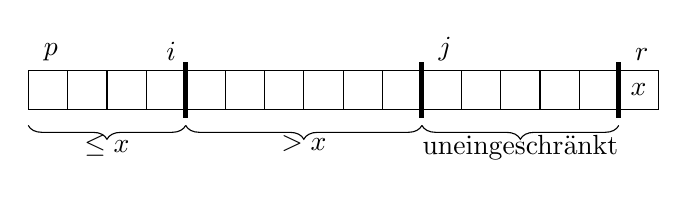
\begin{tikzpicture}
        % Squares
        \draw []    (0.0, 0.0) rectangle (0.5, 0.5) node[above left]{$p$};
        \draw []    (0.5, 0.0) rectangle (1.0, 0.5);
        \draw []    (1.0, 0.0) rectangle (1.5, 0.5);
        \draw []    (1.5, 0.0) rectangle (2.0, 0.5) node[above left]{$i$};

        \draw []    (2.0, 0.0) rectangle (2.5, 0.5);
        \draw []    (2.5, 0.0) rectangle (3.0, 0.5);
        \draw []    (3.0, 0.0) rectangle (3.5, 0.5);
        \draw []    (3.5, 0.0) rectangle (4.0, 0.5);
        \draw []    (4.0, 0.0) rectangle (4.5, 0.5);
        \draw []    (4.5, 0.0) rectangle (5.0, 0.5);

        \draw []    (5.0, 0.0) rectangle (5.5, 0.5) node[above left]{$j$};
        \draw []    (5.5, 0.0) rectangle (6.0, 0.5);
        \draw []    (6.0, 0.0) rectangle (6.5, 0.5);
        \draw []    (6.5, 0.0) rectangle (7.0, 0.5);
        \draw []    (7.0, 0.0) rectangle (7.5, 0.5);
        \draw []    (7.5, 0.0) rectangle (8.0, 0.5);
        \draw []    (7.5, 0.0) rectangle (8.0, 0.5) node[midway]{$x$} node[above left]{$r$};

        % Separators
        \draw[fill=black] (1.975, -0.1) rectangle (2.025, 0.6);
        \draw[fill=black] (4.975, -0.1) rectangle (5.025, 0.6);
        \draw[fill=black] (7.475, -0.1) rectangle (7.525, 0.6);
        
        % Braces
        \draw[decorate, decoration={brace, mirror, amplitude=5pt}]  (0.0, -0.2) -- node[below]{$\leq x$} (2.0, -0.2);
        \draw[decorate, decoration={brace, mirror, amplitude=5pt}]  (2.0, -0.2) -- node[below]{$> x$} (5.0, -0.2);
        \draw[decorate, decoration={brace, mirror, amplitude=5pt}] (5.0, -0.2) -- node[below]{uneingeschränkt} (7.5, -0.2);
    \end{tikzpicture}

    \caption{Die vier Regionen, die von $\proc{Partition}$ auf einem Subarray $A[p \twodots r]$ behandelt werden. Die Werte in $A[p \twodots i]$ sind alle $\leq x$, die Werte in $A[i + 1 \twodots j - 1]$ sind alle $> x$, und $A[r] = x$. Das Subarray $A[j \twodots r - 1]$ kann jegliche Werte beinhalten. Die Abbildung und Beschreibung wurden aus \cite[173]{clrs2001}, Abbildung 7.2 übernommen.}
    \label{fig:quicks-partitioning}
\end{figure}

\begin{codebox}
    \Procname{$\text{Quicksort}(A, p, r)$}
    \li \If $p < r$
    \li     \Then
                $q \gets \text{Partition}(A, p, r)$
    \li         $\text{Quicksort}(A, p, q - 1)$
    \li         $\text{Quicksort}(A, q + 1, r)$
            \End
\end{codebox}

Der tatsächliche Sortieralgorithmus, Quicksort, besteht nun nurmehr aus rekursiven Aufrufen von sich selbst, und damit Partition.

\text{Quicksort} und \text{Partition} sind aus \cite[171]{clrs2001} entnommen. Eine Implementation des ersteren ist in \prettyref{lst:quick} zu finden, letzterer Algorithmus ist äquivalent zu \lstinline{std::partition} (vgl. \cite[927]{ISO-C++17}).

Die Laufzeit von Quicksort hängt von der Aufteilung der Eingabemenge, welche in $\text{Partition}$ geschieht, ab. Im ungünstigsten Fall produziert $\text{Partition}$ ein Subarray mit $n - 1$ Elementen, und eines mit $0$ Elementen. Die Rekursionsgleichung für die Laufzeit ist in diesem Fall
\begin{equation}\label{eq:quicks-efficiency}
\begin{split}
    T(n) &= T(n - 1) + T(0) + O(n)\\
    &= T(n - 1) + O(n)
\end{split}
\end{equation}
nachdem $\text{Partition}$ $O(n)$ ist und ein Aufruf mit einer Menge der Größe $0$ eine Laufzeit von $O(1)$ hat (vgl. \cite[175]{clrs2001}). Daraus folgt eine Effizienz von $O(n^2)$ im schlechtesten Fall (vgl. \cite[49]{rp2013}). Diese Laufzeit tritt auch auf, wenn die Eingabemenge bereits sortiert ist (vgl. \cite[175]{clrs2001}).

Im günstigsten Fall produziert $\text{Partition}$ ein Subarray der Größe $\floor{n/2}$ und eines der Größe $\ceil{n/2} - 1$. In diesem Fall ist die (vereinfachte) Rekursionsgleichung
\begin{equation*}
    T(n) = 2T(n/2) + O(n),
\end{equation*}
mit der Lösung $T(n) = O(n \log n)$ nach \cite[94]{clrs2001}.

\section{Heapsort}
\label{sec:alg-selection}

Unter dem Begriff \enquote{Heap} wird im Folgenden eine in einem Array abgebildete Datenstruktur verstanden, welche als nahezu vollständiger Binärbaum betrachtet werden kann (vgl. \cite[87f]{ahu1974}, siehe \prettyref{fig:heap-tree-array-view}). Stellt ein Array $A$ einen Heap dar, so hat es neben dem bekannten Attribut $\attrib{A}{length}$ ein Attribut $\attrib{A}{heap-size}$, was der Anzahl der Arrayelemente entspricht, die einen Knoten darstellen. Nur die Elemente in $A[1 \twodots \attrib{A}{heap-size}]$ sind gültige Elemente des Heaps, $A[\attrib{A}{heap-size} + 1 \twodots \attrib{A}{length}]$ kann beliebige Elemente enthalten. Diese Notation und Eigenschaften sind äquivalent zu jenen in \cite{clrs2001}.

Es gibt zwei Arten von binären Heaps: Max-Heaps und Min-Heaps. Beide Arten erfüllen eine \enquote{Heap-Eigenschaft}, die von der Art des Heaps abhängig ist. In einem Max-Heap ist dies die \emph{Max-Heap-Eigenschaft}, die aussagt, dass für jeden Knoten $i$, der nicht der Wurzelknoten ist, $A[\text{Parent}(i)] \leq A[i]$ gelten muss (vgl. \cite[92]{hsr1997}). Das heißt, der Wert eines Knotens ist höchstens der seines Elternknotens, das größte Element eines Max-Heaps ist der Wurzelknoten. Min-Heaps werden im Folgenden nicht verwendet und deshalb nicht näher behandelt.

Die \emph{Höhe} eines Knotens in einem Heap ist definiert durch die Anzahl der Kanten entlang des längsten, einfachen Weges zu einem Blattknoten (vgl. \cite[153]{clrs2001}). Die Höhe eines Heaps ist die Höhe des Wurzelknotens (siehe \prettyref{fig:heap-array-view}).

\begin{figure}[htb]
    \centering
    \begin{subfigure}[t]{0.48\linewidth}{\footnotesize
        \centering
        \begin{forest}
            for tree={
                circle, draw,
                minimum size=2em
            }
            [16, very thick, label=1
                [11,  label=2
                    [10,  label=4
                        [1, for ancestors={edge=very thick}, edge=very thick,  label=8]
                        [2,  label=9]
                    ]
                    [5,  label=5
                        [4,  label=10]
                        [,color=white, edge=white]
                    ]
                ]
                [9,  label=3
                    [6,  label=6]
                    [8,  label=7]
                ]
            ]
        \end{forest}

        \subcaption{Der Wurzelknoten und die Kanten entlang eines der längsten, einfachen Wege zu einem Blattknoten sind fett gedruckt. Die Anzahl der hervorgehobenen Kanten entspricht der Höhe $h = 3$ des Baums. \label{fig:heap-tree-view}}
    }\end{subfigure}\hfill
    \begin{subfigure}[t]{0.48\linewidth}{\footnotesize
        \centering
        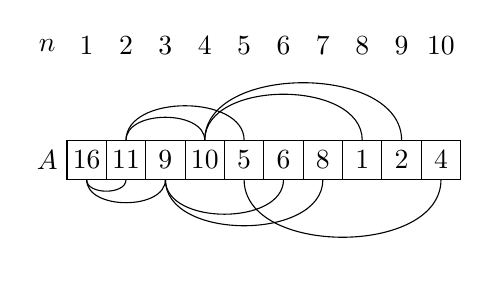
\begin{tikzpicture}
            \path node at (-0.25, 1.25) [] {$A$};
        
            \draw (0.0, 1.0) rectangle (0.5, 1.5) node[midway]{16};
            \draw (0.5, 1.0) rectangle (1.0, 1.5) node[midway]{11};
            \draw (1.0, 1.0) rectangle (1.5, 1.5) node[midway]{9};
            \draw (1.5, 1.0) rectangle (2.0, 1.5) node[midway]{10};
            \draw (2.0, 1.0) rectangle (2.5, 1.5) node[midway]{5};
            \draw (2.5, 1.0) rectangle (3.0, 1.5) node[midway]{6};
            \draw (3.0, 1.0) rectangle (3.5, 1.5) node[midway]{8};
            \draw (3.5, 1.0) rectangle (4.0, 1.5) node[midway]{1};
            \draw (4.0, 1.0) rectangle (4.5, 1.5) node[midway]{2};
            \draw (4.5, 1.0) rectangle (5.0, 1.5) node[midway]{4};

            \draw []   (0.25, 1.0) to[out=-90,in=-90] (0.75, 1.0);
            \draw []   (0.25, 1.0) to[out=-90,in=-90] (1.25, 1.0);
            \draw []   (0.75, 1.5) to[out=90,in=90] (1.75, 1.5);
            \draw []   (0.75, 1.5) to[out=90,in=90] (2.25, 1.5);
            \draw []   (1.25, 1.0) to[out=-90,in=-90] (2.75, 1.0);
            \draw []   (1.25, 1.0) to[out=-90,in=-90] (3.25, 1.0);
            \draw []   (1.75, 1.5) to[out=90,in=90] (3.75, 1.5);
            \draw []   (1.75, 1.5) to[out=90,in=90] (4.25, 1.5);
            \draw []   (2.25, 1.0) to[out=-90,in=-90] (4.75, 1.0);
            
            \path   node at (-0.25, 2.7) [] {$n$}
                    node at (0.25, 2.7) [] {1}
                    node at (0.75, 2.7) [] {2}
                    node at (1.25, 2.7) [] {3}
                    node at (1.75, 2.7) [] {4}
                    node at (2.25, 2.7) [] {5}
                    node at (2.75, 2.7) [] {6}
                    node at (3.25, 2.7) [] {7}
                    node at (3.75, 2.7) [] {8}
                    node at (4.25, 2.7) [] {9}
                    node at (4.75, 2.7) [] {10};
        \end{tikzpicture}
        
        \subcaption{Die Linien über und unter dem Array stellen die Eltern-Kind-Beziehungen zwischen den Knoten dar, Eltern sind immer links von ihren Kindern. \label{fig:heap-array-view}}
    }\end{subfigure}
    \caption{Ein binärer Max-Heap, dargestellt \subref{fig:heap-tree-view} als Binärbaum und \subref{fig:heap-array-view} als Array (wobei $\attrib{A}{heap-size}$ gleich $\attrib{A}{length}$ ist). Die Zahlen in den Kreisen und Rechtecken sind der Wert dieses Knotens beziehungsweise dieses Elements, die Zahlen darüber sind der Index des jeweiligen Knotens/Elements im Array. Angelehnt an \cite[152]{clrs2001} und \cite[88]{ahu1974}.}
    \label{fig:heap-tree-array-view}
\end{figure}

\pagebreak[4]

\paragraph{Aufrechterhaltung eines Heaps}

$\text{Max-Heapify}$ erhält ein Array $A$ und einen index $i$ im Array. Es nimmt an, dass
\begin{itemize}
    \item die Binärbäume links und rechts von $A[i]$ bereits Heaps sind aber dass,
    \item $A[i]$ kleiner als seine Kinder sein könnte, und damit die Heap-Eigenschaft verletzen würde.
\end{itemize}

\begin{minipage}{\textwidth}
    \begin{minipage}[t]{.33\textwidth}
        \begin{codebox}
            \Procname{$\text{Parent}(i)$}
            \li \Return $\floor{i/2}$
        \end{codebox}
    \end{minipage}
    \begin{minipage}[t]{.33\textwidth}
        \begin{codebox}
            \Procname{$\text{Left}(i)$}
            \li \Return $2i$
        \end{codebox}
    \end{minipage}
    \begin{minipage}[t]{.33\textwidth}
        \begin{codebox}
            \Procname{$\text{Right}(i)$}
            \li \Return $2i + 1$
        \end{codebox}
    \end{minipage}
\end{minipage}

Die Hilfsalgorithmen $\text{Parent}$, $\text{Left}$ und $\text{Right}$ sind aus \cite[152]{clrs2001} entnommen.

\begin{codebox}
    \Procname{$\text{Max-Heapify}(A, i)$}
    \li $l \gets \text{Left}(i)$\label{ln:heapify-get-largest-begin}
    \li $r \gets \text{Right}(i)$
    \li \If $l \leq \attrib{A}{heap-size}$ and $A[l] > A[i]$
    \li      \Then
                $\id{largest} \gets l$
    \li     \Else
                $\id{largest} \gets i$
            \End
    \li \If $r \leq \attrib{A}{heap-size}$ and $A[r] > A[\id{largest}]$
    \li     \Then
                $\id{largest} = r$
            \End\label{ln:heapify-get-largest-end}
    \li \If $largest \neq i$ \label{ln:heapify-largest}
    \li     \Then
                exchange $A[i]$ with $A[\id{largest}]$\label{ln:heapify-exchange}
    \li         $\text{Max-Heapify}(A, \id{largest})$\label{ln:heapify-recursion}
            \End
\end{codebox}

Im Laufe der rekursiven Aufrufe an $\text{Max-Heapify}$ \enquote{gleitet} das Element $A[i]$ den Heap hinunter bis die Heap-Eigenschaft gegeben ist: Zeilen \ref{ln:heapify-get-largest-begin} bis \ref{ln:heapify-get-largest-end} ermitteln das größte Element $A[largest]$ aus $\{\text{Left}(i), \text{Right}(i), A[i]\}$. Ist $\text{Left}(i)$ oder $\text{Right}(i)$ nicht Teil des Heaps -- gilt also $\text{Left}(i)$ oder $\text{Right}(i) \leq \attrib{A}{heap-size}$ -- so ist $A[i]$ garantiert das größte Element. Ist $A[largest]$ gleich $A[i]$ dann ist der Baum ab $A[i]$ ein Max-Heap und $\text{Max-Heapify}$ terminiert. Andernfalls werden das größte Element und $A[i]$ vertauscht, wodurch die Heap-Eigenschaft wieder gilt (Zeile \ref{ln:heapify-exchange}). Der Baum ab $A[largest]$ könnte nun jedoch gegen die Heap-Eigenschaft verstoßen (nachdem $A[largest]$ und $A[i]$ vertauscht wurden), also wird $\text{Max-Heapify}$ rekursiv auf diesem \enquote{Unterbaum} aufgerufen (Zeile \ref{ln:heapify-recursion}).

Im ungünstigsten Fall muss der ganze Teilbaum, welcher den Knoten $i$ als Wurzel hat, durchlaufen werden. Ist $n$ die Größe dieses Teilbaums, kann die Höhe des Baums mit $h = \log n$ ermittelt werden, somit ist die Effizienz im ungünstigsten Fall in $O(\log n)$ (vgl. \cite[155]{clrs2001}). Der Einfachheit halber wird diese Effizienz auch für den günstigsten Fall übernommen, eine asymptotisch engere (aber deswegen nicht richtigere) Effizienz wird in \cite{bff1996} angeführt.

\paragraph{Bauen eines Heaps}

Stellt das Array $A$ einen Heap dar, so sind die Elemente $A[\floor{n / 2} + 1 \twodots n]$ Blattknoten des Baumes\footnotemark. $\text{Build-Max-Heap}$ führt für die Knoten $A[1 \twodots \floor{n / 2}]$ $\text{Max-Heapify}$ aus und baut so einen vollständigen Heap aus einem beliebigen Array.

\footnotetext{
Die Kinder eines Knotens an der Stelle $i$ sind an den Stellen $2i$ und $2i + 1$ (siehe $\text{Left}$ und $\text{Right}$). Alle Knoten, die keine Blattknoten sind (d. h., die Eltern sind), müssen sich demzufolge an den Stellen $A[1 \twodots \floor{n / 2}]$ befinden, da ihre Kinder sonst außerhalb des Heaps wären: Ist $i > \floor{n / 2}$ dann wäre $2i > n$ also muss der Knoten an der Stelle $i$ ein Blattknoten sein. (Q. e. d., damit ist Aufgabe 6.1-7 aus \cite[154]{clrs2001} gelöst.)
}

\begin{codebox}
    \Procname{$\text{Build-Max-Heap}(A)$}
    \li $\attrib{A}{heap-size} \gets \attrib{A}{length}$
    \li \For $i \gets \lfloor \attrib{A}{length}/2 \rfloor$ \Downto $1$
    \li     \Do
                $\text{Max-Heapify}(A, i)$
            \End
\end{codebox}

Die Effizienz von $\text{Build-Max-Heap}$ ist immer in $O(n)$, \cite[155]{taocp3} zeigt die Nontrivialität dieser Aussage.

\paragraph{Heapsort}

Die Eingangsmenge $A[1 \twodots n]$ wird mithilfe von $\text{Build-Max-Heap}$ in einen Heap verwandelt. $A[1]$ beinhaltet nun das größte Element der Liste, durch Austauschen von $A[1]$ und $A[n]$ befindet sich das Element bereits an seiner finalen Position. Das bereits einsortierte Element kann nun durch Verkleinerung des Heaps um $1$ von diesem entfernt werden. Das neue Wurzelement könnte jetzt jedoch die Heap-Eigenschaft verletzen, was durch einen Aufruf von $\text{Max-Heapify}$ am Wurzelelement unmöglich gemacht wird.

\begin{codebox}
    \Procname{$\text{Heapsort}(A)$}
    \li $\text{Build-Max-Heap}(A)$
    \li \For $i = \attrib{A}{length}$ \Downto $2$
    \li     \Do
                exchange $A[1]$ with $A[i]$
    \li         $\attrib{A}{heap-size} \gets \attrib{A}{heap-size} - 1$
    \li         $\text{Max-Heapify(A, 1)}$
            \End
\end{codebox}

$\text{Max-Heapify}$, $\text{Build-Max-Heap}$ und $\text{Heapsort}$ sind aus \cite[154, 157]{clrs2001} entnommen. Die Standardbibliothek von C++ deckt die obigen Algorithmen sehr gut ab: $\text{Build-Max-Heap}$ ist äquivalent zu \lstinline{std::make_heap} (vgl. \cite[933]{ISO-C++17}), $\text{Heap\-sort}$ (ohne dem Aufruf von $\text{Build-Max-Heap}$) ist äquivalent zu  \lstinline{std::sort_heap} (vgl. \cite[933]{ISO-C++17}.). \prettyref{lst:heap} ist eine \enquote{Implementation} der obigen Algorithmen -- sie ruft lediglich die eben genannten Funktionen der Standardbibliothek in Folge auf.

Die Effizienz von $\text{Heapsort}$ ist in jedem Fall in $O(n \log n)$ nachdem jeder der $n - 1$ Aufrufe an $\text{Max-Heapify}$ in $O(\log n)$ ist (vgl. \cite[160]{clrs2001}).

\section{Mergesort}
\label{sec:alg-merging}

Mergesort ist, wie der Quicksort ein divide-and-conquer Algorithmus: ein Problem wird in kleinere Subprobleme aufgeteilt, die Lösungen der Subprobleme werden (oft rekursiv) ermittelt und zusammengesetzt.

Die entscheidende Handlung ist beim Mergesort das Kombinieren (nicht wie beispielsweise beim Quicksort das Aufteilen), welches in $\text{Merge}$ durchgeführt wird.

\begin{codebox}
    \Procname{$\text{Merge}(A, p, q, r)$}
    \li $n_1 \gets q - p + 1$ \label{ln:merge-subarr-length-1}
    \li $n_2 \gets r - q$ \label{ln:merge-subarr-length-2}
    \li let $L[1 \twodots n_1 + 1]$ and $R[1 \twodots n_2 + 1]$ be new arrays \label{ln:merge-subarr-creation}
    \li \For $i \gets 1$ \To $n_1$ \label{ln:merge-copy-begin}
    \li     \Do
                $L[i] \gets A[p + i - 1]$
            \End
    \li \For $j \gets 1$ \To $n_2$ \label{ln:merge-copy-for-2}
    \li     \Do
                $R[j] \gets A[q + j]$
            \End \label{ln:merge-copy-end}
    \li $L[n_1 + 1] \gets \infty$ \label{ln:merge-infty-assign-1}
    \li $R[n_2 + 1] \gets \infty$ \label{ln:merge-infty-assign-2}
    \li $i \gets 1$
    \li $j \gets 1$ \label{ln:merge-index-setup-2}
    \li \For $k \gets p$ \To $r$ \label{ln:merge-for-begin}
    \li     \Do
                \If $L[i] \leq R[j]$
                    \Then
    \li                 $A[k] \gets L[i]$
    \li                 $i \gets i + 1$
                    \Else
                        $A[k] \gets R[j]$
    \li                 $j \gets j + 1$
                    \End
            \End \label{ln:merge-for-end}
\end{codebox}

$\text{Merge}$ mag auf den ersten Blick komplex wirken, es kann jedoch in einfache Phasen heruntergebrochen werden:
\begin{enumerate}[start=0]
    \item $p$, $q$ und $r$ sind Indices des Eingabearrays $A$, es gilt $p \leq q < r$. Es wird angenommen, dass die Subarrays $A[r \twodots q]$ und $A[q + 1 \twodots r]$ sortiert sind.

    \item Erstelle ein Array $L$ mit den Werten $A[r \twodots q]$ und ein Array $R$ mit den Werten $A[q + 1 \twodots r]$. Hänge $\infty$ an beide Arrays an. \emph{(Zeilen \ref{ln:merge-subarr-length-1} bis \ref{ln:merge-infty-assign-2})}

    \item Assoziiere mit dem Array $L$ einen Index $i$ und mit dem Array $R$ einen Index $j$. Beide beginnen bei $1$, jegliche Zugriffe auf $L$ und $R$ geschehen von nun an nur über diese Indices. Durch Erhöhen eines der Indices können nun Elemente de facto aus dem Array entfernt werden. \emph{(Zeilen \ref{ln:merge-infty-assign-1} und \ref{ln:merge-infty-assign-2})}

    \item Iteriere über alle Elemente des Arrays $A$:

    Ist $L[i] \leq R[j]$ so wird das aktuelle Element aus $A$ mit $L[i]$ überschrieben. $L[i]$ ist nun einsortiert, $i$ wird um $1$ erhöht. Andernfalls wird das aktuelle Element aus $A$ mit $R[j]$ überschrieben und $j$ um eins erhöht. \emph{(Zeilen \ref{ln:merge-for-begin} bis \ref{ln:merge-for-end})}

    Wird ein Array \enquote{erschöpft}, wurden also alle seine ursprünglich aus $A$ stammenden Elemente einsortiert, so zeigt der jeweilige Index auf $\infty$. Dieses Element kann niemals einsortiert werden, nachdem kein Element von $L$ oder $R$ jemals $< \infty$ sein kann, zeigt ein Index eines Subarrays darauf, wird dieses also de facto ignoriert. Durch dieses \enquote{Scheinelement} muss nicht bei jeder Iteration überprüft werden, ob eines der Arrays leer ist.
\end{enumerate}

Die Effizienz der $\text{Merge}$-Prozedur ist immer in $O(n)$, nachdem die Anweisungen auf Zeilen \ref{ln:merge-subarr-length-1}--\ref{ln:merge-subarr-creation} und \ref{ln:merge-infty-assign-1}--\ref{ln:merge-index-setup-2} konstante Zeit benötigen und die $\For$-Schleifen auf Zeilen \ref{ln:merge-copy-begin}--\ref{ln:merge-copy-end} und \ref{ln:merge-for-begin}--\ref{ln:merge-for-end} alle anschaulicherweise in $O(n)$ sind (vgl. \cite[34]{clrs2001}).

Um nun ein Array $A$ zu sortieren wird $\text{Mergesort}(A, 1, \attrib{A}{length})$ aufgerufen. $\text{Mergesort}$ halbiert das Eingangsarray durch rekursive Aufrufe bis nur mehr Subarrays der Größe 1 übrig bleiben. Diese Subarrays werden anschließlich durch den auf die rekursiven Aufrufe folgenden Aufruf von $\text{Merge}$ in sukzessiv größere Subarrays zusammengefügt bis ein sortiertes Array als Resultat des letzten Aufrufs hervorgeht.

\begin{codebox}
    \Procname{$\text{Mergesort}(A, p, r)$}
    \li \If $p < r$
    \li     \Do
                $q \gets \floor{(p + r) / 2}$\label{ln:merges-division-begin}
    \li         $\text{Merge-Sort}(A, p, q)$\label{ln:merges-recusion-begin}
    \li         $\text{Merge-Sort}(A, q + 1, r)$\label{ln:merges-division-end}\label{ln:merges-recusion-end}
    \li         $\text{Merge}(A, p, q, r)$
            \End
\end{codebox}

$\text{Merge}$ und $\text{Mergesort}$ sind aus \cite[33f]{clrs2001} entnommen. $\text{Merge}$ ist äquivalent zu \lstinline{std::inplace_merge} (vgl. \cite[929]{ISO-C++17}), eine Implementation von $\text{Mergesort}$ ist in \prettyref{lst:merge} zu finden.

Unter der Annahme, dass $n$ eine Zweierpotenz ist, liefert jeder Teilungsschritt (Zeilen \ref{ln:merges-division-begin}--\ref{ln:merges-division-end}) zwei Subarrays der Größe $n / 2$. Jeder Rekursionsschritt (Zeilen \ref{ln:merges-recusion-begin}--\ref{ln:merges-recusion-end}) trägt also $2T(n / 2)$ zur Effizienz bei (\cite[36]{clrs2001}).

Wie auch schon bei $\text{Quicksort}$ kann die Effizienz des $\text{Mergesort}$ durch eine Rekursionsgleichung
\begin{equation}\label{eq:merge-sort-recurrence}
    T(n) = \begin{cases}
        O(1), & \text{wenn $n = 1$},\\
        2T(n/2) + O(n), & \text{wenn $n > 1$}.
    \end{cases}
\end{equation}
beschrieben werden (vgl. \cite[36]{clrs2001}). Der Summand $O(n)$ ist hier die Effizienz von $\text{Merge}$. \eqref{eq:merge-sort-recurrence} deckt sich mit \eqref{eq:quicks-efficiency}, sowohl im günstigsten als auch im ungünstigsten Fall, damit ist die Effizienz von $\text{Quicksort}$ in $O(n \log n)$ (vgl. \cite[36]{clrs2001}).
